\section{Extension to Multiple Categories}

We present here how the methodology described in Section~\ref{inference_methodology} for
two categories can be extended to multiple categories.
To this end, we separate the income values into five distinct groups $ H_1, \ldots, H_5 \subseteq G$ of increasing wealth. A user is part of this group if its income is between the defined bounds, that is, \( g \in H_i \iff g_s \in R_i \).

The income ranges are set as follows (in Mexican pesos):
	$R_1 = \left[1000, 2500\right) $;
	$R_2 = \left[2500, 7500\right) $;
	$R_3 = \left[7500, 20000\right) $;
	$R_4 = \left[20000, 50000\right) $;
	$R_5 = \left[50000, \infty\right) $.

Again, we define the set $Q$ as the group of users having at least one connection link to bank clients. For each user $q^j \in Q$, we compute the number of outgoing calls $a^j_i$ to the category $H_i$.
We use the amount of calls $a^j_i$  as parameters defining a Dirichlet distribution for the probability of belonging to each category.
We define below the Dirichlet probability distribution function $D^j$:
\begin{equation}
D^j \left( x_1, \ldots, x_5; \alpha^j_1, \ldots, \alpha^j_5 \right) = \frac{1}{\Beta \left( \alpha \right)} \prod^5_{i = 1} x_i^{\alpha^j_i - 1}
\label{Dirichlet}
\end{equation}
where $\alpha^j_i = a^j_i +1$ are the parameters of the Dirichlet distribution, and $\Beta$ is the multivariate beta distribution function, defined by: % (\eqref{Beta})
\begin{equation}
\Beta \left( \alpha_1, \ldots, \alpha_k \right) = \frac{\prod^k_{i = 1} \Gamma \! \left( \alpha_i \right)}{\Gamma \! \left( \sum^k_{i = 1} \alpha_i \right) }
\label{Beta}
\end{equation}

Note that the above equation defines a distinct Dirichlet distribution for each user. For each of these distributions, we computed the marginal probability functions across all different categories, which result in Beta distributed functions, and use them to get the lowest 5 percentiles (\(p^i_{\operatorname{lower}}\)) in each case ${i=1, \ldots, 5}$ which can be compared to assign a category to each user.

\begin{figure}
\centering
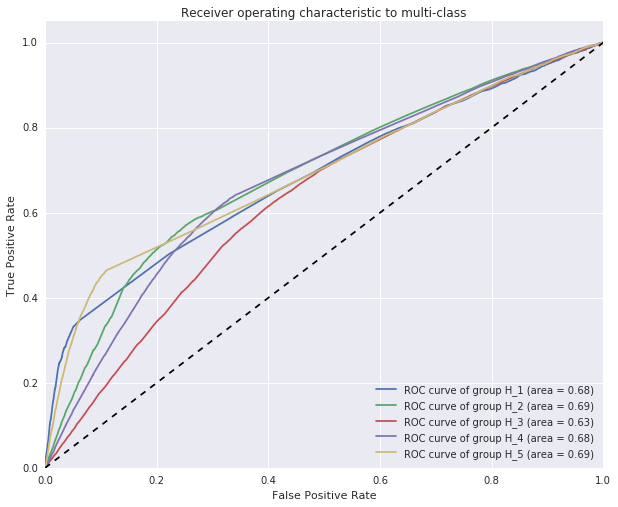
\includegraphics[width=0.75\columnwidth]{figures/ROC_multiclass/ROC_multiclass.png}
\caption{ROC curves for multiclass problem. The performances observed are: $\AUC_1 = 0.68$, $\AUC_2 = 0.69$, $\AUC_3 = 0.63$, $\AUC_4 = 0.68$, $\AUC_5 = 0.69$. These predictors perform better than the random case, and have a similar performance (with exception of category 3).}
\label{roc_multiple_categories}
\end{figure}

In order to gain an intuition on how the classification extends to the multiple category case, we constructed for each category $i$ a binary classifier by using the computed $p^i_{lower}$ score and a given threshold $\tau$. In each case we sweep the threshold $\tau$ and compute the resulting ROC curves as shown in Figure~\ref{roc_multiple_categories}.

We observed the performance for the different categories: $\AUC_1 = 0.68$, $\AUC_2 = 0.69$, $\AUC_3=0.63$, $\AUC_4 = 0.68$, $\AUC_5 = 0.69$. In all cases, the predictor performs better than the random case.

%It is worth of mention that in this last case, the income range $[7500,20000]$) matches cualitatively with the range were dispersion in the heatmap get broader (see figure \ref{homophily_heatmap}). This suggest that for this range of income it would be useful to complement the proposed approach with other orthogonal income information or prediction strategies, as users geolocalization, credit card debts, etc.

%We use the Dirichlet distribution to define the following algorithm to infer the appropriate income category for each user
